\documentclass [11pt, a4wide, twoside]{article}

\usepackage{times}
\usepackage{epsfig}
\usepackage{ifthen}
\usepackage{xspace}
\usepackage{fancyhdr}
\usepackage[colorlinks = true,linkcolor = black,urlcolor  = blue,citecolor = black,anchorcolor = black]{hyperref}
\usepackage{verbatim}
\usepackage{amsmath}
\usepackage{graphicx}

\usepackage{listings}
\usepackage{color}
%\usepackage{enumitem}

\definecolor{dkgreen}{rgb}{0,0.6,0}
\definecolor{gray}{rgb}{0.5,0.5,0.5}
\definecolor{mauve}{rgb}{0.58,0,0.82}

\lstset{frame=tb,
language=Java,
aboveskip=3mm,
belowskip=3mm,
showstringspaces=false,
columns=flexible,
basicstyle={\small\ttfamily},
numbers=none,
numberstyle=\tiny\color{gray},
keywordstyle=\color{blue},
commentstyle=\color{dkgreen},
stringstyle=\color{mauve},
breaklines=true,
breakatwhitespace=true
tabsize=3
}

\newboolean{showsolution}
\setboolean{showsolution}{true} 

% \newlist{todolist}{itemize}{2}
% \setlist[todolist]{label=$\square$}
% \usepackage{pifont}
% \newcommand{\cmark}{\ding{51}}%
% \newcommand{\xmark}{\ding{55}}%
% \newcommand{\done}{\rlap{$\square$}{\raisebox{2pt}{\large\hspace{1pt}\cmark}}%
% \hspace{-2.5pt}}
% \newcommand{\wontfix}{\rlap{$\square$}{\large\hspace{1pt}\xmark}}


% \usepackage{times}
\usepackage{epsfig}
\usepackage{ifthen}
\usepackage{xspace}
\usepackage{fancyhdr}
\usepackage{amsthm}
\usepackage{hyperref}



%layout
\topmargin      -5.0mm
\oddsidemargin  6.0mm
\evensidemargin -6.0mm
\textheight     215.5mm
\textwidth      160.0mm
\parindent      1.0em
\headsep        10.3mm
\headheight     12pt
\lineskip       1pt
\normallineskip 1pt

\newtheorem{mydef}{Definition}


%header
\lhead{Software Modeling and Analysis \\ 2016}

\rhead{Prof. Oscar Nierstrasz, Mohammad Ghafari, Nevena Milojkovi\'{c} and Yuriy Tymchuk}

\lfoot{page \thepage}
\rfoot{\today}
\cfoot{}

\renewcommand{\headrulewidth}{0.1pt}
\renewcommand{\footrulewidth}{0.1pt}

%enumeration
\newenvironment{myitemize}{%
     \begin{itemize}
     \setlength{\itemsep}{0cm}}
     {\end{itemize}}

\newenvironment{myenumerate}{%
     \begin{enumerate} \setlength{\itemsep}{0cm}}
     {\end{enumerate}}


%solution
\ifthenelse{\boolean{showsolution}}
   {  \newcommand{\solution}[1]{
   	\noindent\underline{\textbf{Answer:}}\\[2mm]
   	 \textsl{#1}
	 \vspace{10pt}
	 \normalsize
	}
  }
  {  \newcommand{\solution}[1]{} }


\pagestyle{fancy}

% ============================================================
% Markup macros for proof-reading
\usepackage{ifthen}
\usepackage[normalem]{ulem} % for \sout
\usepackage{xcolor}
\newcommand{\ra}{$\rightarrow$}
\newboolean{showedits}
\setboolean{showedits}{true} % toggle to show or hide edits
\ifthenelse{\boolean{showedits}}
{
	\newcommand{\ugh}[1]{\textcolor{red}{\uwave{#1}}} % please rephrase
	\newcommand{\ins}[1]{\textcolor{blue}{\uline{#1}}} % please insert
	\newcommand{\del}[1]{\textcolor{red}{\sout{#1}}} % please delete
	\newcommand{\chg}[2]{\textcolor{red}{\sout{#1}}{\ra}\textcolor{blue}{\uline{#2}}} % please change
}{
	\newcommand{\ugh}[1]{#1} % please rephrase
	\newcommand{\ins}[1]{#1} % please insert
	\newcommand{\del}[1]{} % please delete
	\newcommand{\chg}[2]{#2}
}
% ============================================================
% Put edit comments in a really ugly standout display
%\usepackage{ifthen}
\usepackage{amssymb}
\newboolean{showcomments}
\setboolean{showcomments}{true}
%\setboolean{showcomments}{false}
\newcommand{\id}[1]{$-$Id: scgPaper.tex 32478 2010-04-29 09:11:32Z oscar $-$}
\newcommand{\yellowbox}[1]{\fcolorbox{gray}{yellow}{\bfseries\sffamily\scriptsize#1}}
\newcommand{\triangles}[1]{{\sf\small$\blacktriangleright$\textit{#1}$\blacktriangleleft$}}
\ifthenelse{\boolean{showcomments}}
%{\newcommand{\nb}[2]{{\yellowbox{#1}\triangles{#2}}}
{\newcommand{\nbc}[3]{
 {\colorbox{#3}{\bfseries\sffamily\scriptsize\textcolor{white}{#1}}}
 {\textcolor{#3}{\sf\small$\blacktriangleright$\textit{#2}$\blacktriangleleft$}}}
 \newcommand{\version}{\emph{\scriptsize\id}}}
{\newcommand{\nbc}[3]{}
 \renewcommand{\ugh}[1]{#1} % please rephrase
 \renewcommand{\ins}[1]{#1} % please insert
 \renewcommand{\del}[1]{} % please delete
 \renewcommand{\chg}[2]{#2} % please change
 \newcommand{\version}{}}
\newcommand{\nb}[2]{\nbc{#1}{#2}{orange}}
\newcommand{\here}{\yellowbox{$\Rightarrow$ CONTINUE HERE $\Leftarrow$}}
\newcommand\rev[2]{\nb{TODO (rev #1)}{#2}} % reviewer comments
\newcommand\fix[1]{\nb{FIX}{#1}}
\newcommand\todo[1]{\nb{TO DO}{#1}}
\newcommand\on[1]{\nbc{ON}{#1}{red}} % add more author macros here
%\newcommand\XXX[1]{\nbc{XXX}{#1}{blue}}
%\newcommand\XXX[1]{\nbc{XXX}{#1}{brown}}
%\newcommand\XXX[1]{\nbc{XXX}{#1}{cyan}}
%\newcommand\XXX[1]{\nbc{XXX}{#1}{darkgray}}
%\newcommand\XXX[1]{\nbc{XXX}{#1}{gray}}
%\newcommand\XXX[1]{\nbc{XXX}{#1}{magenta}}
%\newcommand\XXX[1]{\nbc{XXX}{#1}{olive}}
%\newcommand\XXX[1]{\nbc{XXX}{#1}{orange}}
%\newcommand\XXX[1]{\nbc{XXX}{#1}{purple}}
%\newcommand\XXX[1]{\nbc{XXX}{#1}{red}}
%\newcommand\XXX[1]{\nbc{XXX}{#1}{teal}}
%\newcommand\XXX[1]{\nbc{XXX}{#1}{violet}}
%=============================================================
% ST80 listings macros
% Adapted from Squeak by Example book
%=============================================================
% If you want >>> appearing as right guillemet, you need these two lines:
%\usepackage[T1]{fontenc}
%\newcommand{\sep}{\mbox{>>}}
% Otherwise use this:
\newcommand{\sep}{\mbox{$\gg$}}
%=============================================================
%:\needlines{N} before code block to force page feed
\usepackage{needspace}
\newcommand{\needlines}[1]{\Needspace{#1\baselineskip}}
%=============================================================
%:Listings package configuration for ST80
\usepackage[english]{babel}
\usepackage{amssymb,textcomp}
\usepackage{listings}
% \usepackage[usenames,dvipsnames]{color}
% \usepackage[usenames]{color}
% \definecolor{source}{gray}{0.95}
\lstdefinelanguage{Smalltalk}{
%  morekeywords={self,super,true,false,nil,thisContext}, % This is overkill
  morestring=[d]',
  morecomment=[s]{"}{"},
  alsoletter={\#:},
  escapechar={!},
  literate=
    {BANG}{!}1
    {UNDERSCORE}{\_}1
    {\\st}{Smalltalk}9 % convenience -- in case \st occurs in code
    % {'}{{\textquotesingle}}1 % replaced by upquote=true in \lstset
    {_}{{$\leftarrow$}}1
    {>>>}{{\sep}}1
    {^}{{$\uparrow$}}1
    {~}{{$\sim$}}1
    {-}{{\sf -\hspace{-0.13em}-}}1  % the goal is to make - the same width as +
    {+}{\raisebox{0.08ex}{+}}1		% and to raise + off the baseline to match -
    {-->}{{\quad$\longrightarrow$\quad}}3
	, % Don't forget the comma at the end!
  tabsize=4
}[keywords,comments,strings]

\definecolor{source}{gray}{0.95}

\lstset{language=Smalltalk,
	basicstyle=\sffamily,
	keywordstyle=\color{black}\bfseries,
	% stringstyle=\ttfamily, % Ugly! do we really want this? -- on
	mathescape=true,
	showstringspaces=false,
	keepspaces=true,
	breaklines=true,
	breakautoindent=true,
	backgroundcolor=\color{source},
	lineskip={-1pt}, % Ugly hack
	upquote=true, % straight quote; requires textcomp package
	columns=fullflexible} % no fixed width fonts
% In-line code (literal)
% Normally use this for all in-line code:
\newcommand{\ct}{\lstinline[mathescape=false,backgroundcolor=\color{white},basicstyle={\sffamily\upshape}]}
% In-line code (latex enabled)
% Use this only in special situations where \ct does not work
% (within section headings ...):
\newcommand{\lct}[1]{{\textsf{\textup{#1}}}}
% Code environments
\lstnewenvironment{code}{%
	\lstset{%
		% frame=lines,
		frame=single,
		framerule=0pt,
		mathescape=false
	}
}{}

% Useful to add a matching $ after code containing a $
% \def\ignoredollar#1{}
%=============================================================
\newcommand{\ie}{\emph{i.e.}\xspace}
\newcommand{\eg}{\emph{e.g.}\xspace}
\newcommand{\etal}{\emph{et al.}\xspace}
% ============================================================

% \definecolor{mircolor}{rgb}{0.4,0.6,0.2}
% \newcommand\ml[1]{\nbc{ML}{#1}{mircolor}}
% \usepackage{wasysym}
% \newcommand\yesml[1]{\nbc{ML {\textcolor{yellow}\sun}}{#1}{mircolor}}

\usepackage{times}
\usepackage{epsfig}
\usepackage{ifthen}
\usepackage{xspace}
\usepackage{fancyhdr}
\usepackage{amsthm}
\usepackage{hyperref}



%layout
\topmargin      -5.0mm
\oddsidemargin  6.0mm
\evensidemargin -6.0mm
\textheight     215.5mm
\textwidth      160.0mm
\parindent      1.0em
\headsep        10.3mm
\headheight     12pt
\lineskip       1pt
\normallineskip 1pt

\newtheorem{mydef}{Definition}


%header
\lhead{Software Modeling and Analysis \\ 2016}

\rhead{Prof. Oscar Nierstrasz, Mohammad Ghafari, Nevena Milojkovi\'{c} and Yuriy Tymchuk}

\lfoot{page \thepage}
\rfoot{\today}
\cfoot{}

\renewcommand{\headrulewidth}{0.1pt}
\renewcommand{\footrulewidth}{0.1pt}

%enumeration
\newenvironment{myitemize}{%
     \begin{itemize}
     \setlength{\itemsep}{0cm}}
     {\end{itemize}}

\newenvironment{myenumerate}{%
     \begin{enumerate} \setlength{\itemsep}{0cm}}
     {\end{enumerate}}


%solution
\ifthenelse{\boolean{showsolution}}
   {  \newcommand{\solution}[1]{
   	\noindent\underline{\textbf{Answer:}}\\[2mm]
   	 \textsl{#1}
	 \vspace{10pt}
	 \normalsize
	}
  }
  {  \newcommand{\solution}[1]{} }


\pagestyle{fancy}

% ============================================================
% Markup macros for proof-reading
\usepackage{ifthen}
\usepackage[normalem]{ulem} % for \sout
\usepackage{xcolor}
\newcommand{\ra}{$\rightarrow$}
\newboolean{showedits}
\setboolean{showedits}{true} % toggle to show or hide edits
\ifthenelse{\boolean{showedits}}
{
	\newcommand{\ugh}[1]{\textcolor{red}{\uwave{#1}}} % please rephrase
	\newcommand{\ins}[1]{\textcolor{blue}{\uline{#1}}} % please insert
	\newcommand{\del}[1]{\textcolor{red}{\sout{#1}}} % please delete
	\newcommand{\chg}[2]{\textcolor{red}{\sout{#1}}{\ra}\textcolor{blue}{\uline{#2}}} % please change
}{
	\newcommand{\ugh}[1]{#1} % please rephrase
	\newcommand{\ins}[1]{#1} % please insert
	\newcommand{\del}[1]{} % please delete
	\newcommand{\chg}[2]{#2}
}
% ============================================================
% Put edit comments in a really ugly standout display
%\usepackage{ifthen}
\usepackage{amssymb}
\newboolean{showcomments}
\setboolean{showcomments}{true}
%\setboolean{showcomments}{false}
\newcommand{\id}[1]{$-$Id: scgPaper.tex 32478 2010-04-29 09:11:32Z oscar $-$}
\newcommand{\yellowbox}[1]{\fcolorbox{gray}{yellow}{\bfseries\sffamily\scriptsize#1}}
\newcommand{\triangles}[1]{{\sf\small$\blacktriangleright$\textit{#1}$\blacktriangleleft$}}
\ifthenelse{\boolean{showcomments}}
%{\newcommand{\nb}[2]{{\yellowbox{#1}\triangles{#2}}}
{\newcommand{\nbc}[3]{
 {\colorbox{#3}{\bfseries\sffamily\scriptsize\textcolor{white}{#1}}}
 {\textcolor{#3}{\sf\small$\blacktriangleright$\textit{#2}$\blacktriangleleft$}}}
 \newcommand{\version}{\emph{\scriptsize\id}}}
{\newcommand{\nbc}[3]{}
 \renewcommand{\ugh}[1]{#1} % please rephrase
 \renewcommand{\ins}[1]{#1} % please insert
 \renewcommand{\del}[1]{} % please delete
 \renewcommand{\chg}[2]{#2} % please change
 \newcommand{\version}{}}
\newcommand{\nb}[2]{\nbc{#1}{#2}{orange}}
\newcommand{\here}{\yellowbox{$\Rightarrow$ CONTINUE HERE $\Leftarrow$}}
\newcommand\rev[2]{\nb{TODO (rev #1)}{#2}} % reviewer comments
\newcommand\fix[1]{\nb{FIX}{#1}}
\newcommand\todo[1]{\nb{TO DO}{#1}}
\newcommand\on[1]{\nbc{ON}{#1}{red}} % add more author macros here
%\newcommand\XXX[1]{\nbc{XXX}{#1}{blue}}
%\newcommand\XXX[1]{\nbc{XXX}{#1}{brown}}
%\newcommand\XXX[1]{\nbc{XXX}{#1}{cyan}}
%\newcommand\XXX[1]{\nbc{XXX}{#1}{darkgray}}
%\newcommand\XXX[1]{\nbc{XXX}{#1}{gray}}
%\newcommand\XXX[1]{\nbc{XXX}{#1}{magenta}}
%\newcommand\XXX[1]{\nbc{XXX}{#1}{olive}}
%\newcommand\XXX[1]{\nbc{XXX}{#1}{orange}}
%\newcommand\XXX[1]{\nbc{XXX}{#1}{purple}}
%\newcommand\XXX[1]{\nbc{XXX}{#1}{red}}
%\newcommand\XXX[1]{\nbc{XXX}{#1}{teal}}
%\newcommand\XXX[1]{\nbc{XXX}{#1}{violet}}
%=============================================================
% ST80 listings macros
% Adapted from Squeak by Example book
%=============================================================
% If you want >>> appearing as right guillemet, you need these two lines:
%\usepackage[T1]{fontenc}
%\newcommand{\sep}{\mbox{>>}}
% Otherwise use this:
\newcommand{\sep}{\mbox{$\gg$}}
%=============================================================
%:\needlines{N} before code block to force page feed
\usepackage{needspace}
\newcommand{\needlines}[1]{\Needspace{#1\baselineskip}}
%=============================================================
%:Listings package configuration for ST80
\usepackage[english]{babel}
\usepackage{amssymb,textcomp}
\usepackage{listings}
% \usepackage[usenames,dvipsnames]{color}
% \usepackage[usenames]{color}
% \definecolor{source}{gray}{0.95}
\lstdefinelanguage{Smalltalk}{
%  morekeywords={self,super,true,false,nil,thisContext}, % This is overkill
  morestring=[d]',
  morecomment=[s]{"}{"},
  alsoletter={\#:},
  escapechar={!},
  literate=
    {BANG}{!}1
    {UNDERSCORE}{\_}1
    {\\st}{Smalltalk}9 % convenience -- in case \st occurs in code
    % {'}{{\textquotesingle}}1 % replaced by upquote=true in \lstset
    {_}{{$\leftarrow$}}1
    {>>>}{{\sep}}1
    {^}{{$\uparrow$}}1
    {~}{{$\sim$}}1
    {-}{{\sf -\hspace{-0.13em}-}}1  % the goal is to make - the same width as +
    {+}{\raisebox{0.08ex}{+}}1		% and to raise + off the baseline to match -
    {-->}{{\quad$\longrightarrow$\quad}}3
	, % Don't forget the comma at the end!
  tabsize=4
}[keywords,comments,strings]

\definecolor{source}{gray}{0.95}

\lstset{language=Smalltalk,
	basicstyle=\sffamily,
	keywordstyle=\color{black}\bfseries,
	% stringstyle=\ttfamily, % Ugly! do we really want this? -- on
	mathescape=true,
	showstringspaces=false,
	keepspaces=true,
	breaklines=true,
	breakautoindent=true,
	backgroundcolor=\color{source},
	lineskip={-1pt}, % Ugly hack
	upquote=true, % straight quote; requires textcomp package
	columns=fullflexible} % no fixed width fonts
% In-line code (literal)
% Normally use this for all in-line code:
\newcommand{\ct}{\lstinline[mathescape=false,backgroundcolor=\color{white},basicstyle={\sffamily\upshape}]}
% In-line code (latex enabled)
% Use this only in special situations where \ct does not work
% (within section headings ...):
\newcommand{\lct}[1]{{\textsf{\textup{#1}}}}
% Code environments
\lstnewenvironment{code}{%
	\lstset{%
		% frame=lines,
		frame=single,
		framerule=0pt,
		mathescape=false
	}
}{}

% Useful to add a matching $ after code containing a $
% \def\ignoredollar#1{}
%=============================================================
\newcommand{\ie}{\emph{i.e.}\xspace}
\newcommand{\eg}{\emph{e.g.}\xspace}
\newcommand{\etal}{\emph{et al.}\xspace}
% ============================================================


\begin{document}

\section*{\ifthenelse{\boolean{showsolution}}{\textcolor{red}{Solution}\\}{}Assignment 08 --- 04.11.2020 -- v1.0\\Code and Test Smells}

\textcolor{red}{Please submit this exercise by email to \href{mailto:pascal.gadient@inf.unibe.ch}{pascal.gadient@inf.unibe.ch} \underline{before} 11 November 2020, 10:15am.\begin{center}\textbf{You must submit your code as editable text, i.e., use plain text file(s).}\end{center}}

\noindent For the second part of this exercise, we use the latest GT release from \href{https://gtoolkit.com/download/}{here}. If you already imported some Moose (MSE) models from the previous assignments into your GT environment, please start with a fresh copy of GT to reduce the strains on your computer's random access memory.
\\\\
\noindent First, we have to download and extract the \emph{Weka} dataset, and second, we need to import it into GT. We can perform both tasks using GT's Playground. Be warned: this process will take several minutes depending on your device's CPU and internet connection. We strongly advise you to save the image when the process succeeded to avoid redoing these steps.\\

\noindent The datasets can be downloaded and extracted with the following script:\\\\
\texttt{targetFolder := (FileLocator imageDirectory asFileReference / \textquotesingle models\textquotesingle) ensureCreateDirectory.\\
archiveFileName := \textquotesingle weka-3-8.zip\textquotesingle.\\
archiveUrl := \textquotesingle https://dl.feenk.com/moose-tutorial/weka/\textquotesingle.\\
ZnClient new\\
\hspace*{0.5cm}url: archiveUrl, archiveFileName;\\
\hspace*{0.5cm}signalProgress: true;\\
\hspace*{0.5cm}downloadTo: targetFolder.\\
(ZipArchive new\\
\hspace*{0.5cm}readFrom: targetFolder / archiveFileName)\\
\hspace*{0.5cm}extractAllTo: targetFolder.}\\

\noindent The sample dataset can be imported with the following script:\\\\
\texttt{modelFile := (FileLocator imageDirectory asFileReference / \textquotesingle models\textquotesingle)\\
\hspace*{0.5cm}/ \textquotesingle weka-3-8\textquotesingle\\
\hspace*{0.5cm}/ \textquotesingle weka-3-8.mse\textquotesingle.\\
modelWeka := MooseModel new\\
\hspace*{0.5cm}importMSEFromFile: modelFile.}

\newpage

\subsection*{Exercise 1: Code smells (4 pts)}
\begin{enumerate}[a)]
\item Choose \underline{two} different code smells and answer the following questions for each of the smells:\\
Which code smell did you chose? What are its characteristics? What is the resulting problem?\\(2 pts)
\solution{There exist numerous code smells and all of them eventually lead to high technical debt.
We list four of them: \begin{itemize}
\item \textbf{Class Data Should Be Private}: A class exposing its attributes, violating the
information hiding principle. \emph{Problem:} When classes expose more attributes than necessary, information leaks or inappropriate value changes might occur. In addition, the technical complexity increases, e.g., every attribute can become referenced at any location in the code.
\item \textbf{Complex Class}: A class having high cyclomatic complexity. \emph{Problem:} The higher the complexity, the more code paths exist through the class. The more code paths exist, the harder it is for developers to fully understand (and test!) the class.
\item \textbf{Functional Decomposition}: A class where inheritance and polymorphism are poorly used, declaring many fields and implementing few methods. \emph{Problem:} The domain model does not adequately reflect the real world model. Hence, it is cumbersome for developers to maintain the code, because they have to work around many dependencies and think in a counter-intuitive way.
\item \textbf{Spaghetti Code}: A class without a structure that declares long methods without parameters. \emph{Problem: The lack of parameters unevitable leads to shared state (variables) within a class. If methods become longer, they usually use more of those shared variables without clear boundaries. As a result, it is particularly hard to make minor adjustments in such classes, because they might impact the whole class.}
\end{itemize}}

\item What is the fundamental problem in developers' code smell perception? (1 pt)
\solution{The perception is a subjective matter. Hence, it is very difficult for developers to reach an agreement regarding the ``smelliness'' of code. The perception is even highly context dependent, \eg an internal application for cleaning log files is in general less exposed to security threats than web endpoints, thus some smells might become neglected. Moreover, different programmers have different programming habits shaped by their culture, and previous experiences. Hence, a code smell in one project might not be considered as a code smell in another project. \textit{Anaïs Nin} sums it up quite nicely: ``We don't see things as they are, we see things as we are.''}

\item What is \emph{association rule mining} in the context of the HIST code smell paper you can find \href{https://www.computer.org/csdl/proceedings/ase/2013/0215/00/06693086.pdf}{here}?\\(1 pt)
\solution{More general, association rules are the correlations between elements that co-occur frequently within a dataset consisting of multiple independent selections of elements. In the context of the HIST paper, the association rules represent correlations between subsets of methods in the same class that frequently change together. The discovery of all association rules within one or more projects is then called ``association rule mining''.}
\end{enumerate}

\ifthenelse{\boolean{showsolution}}{\newpage}{}

\subsection*{Exercise 2: Test code smells (3 pts)}
\begin{enumerate}[a)]
\item Choose \underline{one} test code smell (except ``Eager Test'') and answer the following questions:\\
Which test code smell did you chose? What are its characteristics? What is the resulting problem?\\(1 pt)
\solution{There exist numerous test code smells and all of them eventually lead to high technical debt.
We list three of them: \begin{itemize}
\item \textbf{Empty Test}: A test without any code. \emph{Problem:} Such tests clutter the results and do not have any purpose. Hence, they should be removed.
\item \textbf{Ignored Test}: A test that is ignored either during or after execution time. \emph{Problem:} Such tests should be revised or removed, because they only add dead code to the project.
\item \textbf{Sleepy Test}: A test that lets the testing thread sleep, e.g., invoking \texttt{Thread.sleep()}. \emph{Problem:} A delayed testing thread can cause several problems. Most prominently, it delays the execution of all remaining tests making it unfeasible to execute them in a timely manner. In addition, such tests that rely on platform-dependent features might yield different results on different platforms.
\end{itemize}}

\item Considering the code below, report in which line you can find the ``Eager Test'' code smell and explain why it represents a problem. (2 pts)\\\\
\texttt{01: public void testDataIsVariable() throws Throwable \{\\
02: \hspace*{0.5cm}JSTerm term = new JSTerm();\\
03: \hspace*{0.5cm}term.makeVariable();\\ 
04: \hspace*{0.5cm}term.add((Object) "");\\
05: \hspace*{0.5cm}jSTerm0.matches(jSTerm0);\\
06: \hspace*{0.5cm}assertEquals(false, term.isGround());\\
07: \hspace*{0.5cm}assertEquals(true, term.isVariable());\\
08: \}}\\\\
\solution{The ``Eager Test'' code smell can be found in line 07. This test uses two different assert statements each testing a different method within the same test case. This complicates not only the implementation of the test, it also misleads developers when the test breaks due to the inappropriate test name, and finally, it makes it harder to fix code that breaks such a test because it is not obvious what the cause of the failure is. Consequently, a single test should use a single \texttt{assert} statement on one specific method call of the class under test.}
\end{enumerate}

%\ifthenelse{\boolean{showsolution}}{\newpage}{}

% \subsection*{Exercise 3: Detection of unreachable root classes (5 pts + 3 pts BONUS)}
% Your task is find and visualize all unreachable root classes in \texttt{modelWeka}. This task consists of four different steps, one after another.

% \begin{enumerate}[{Step} 1)]
% \item Find all methods reachable from main. You can use \texttt{invokedMethods} to find the initial invoked methods, and then you do have to repeat this process until you find no more invoked methods. (2 pts)
% \solution{\texttt{reachableMethods := Set new.\\
% methodsToCheck := (modelWeka allModelMethods select: \\
% \hspace*{0.5cm}[ :m \textbar~m name = \textquotesingle main\textquotesingle~]) entities.\\
% \hspace*{0.0cm}[ methodsToCheck notEmpty ] whileTrue: [ \textbar~m \textbar\\
% \hspace*{0.5cm}m := methodsToCheck removeFirst.\\
% \hspace*{0.5cm}m invokedMethods do: [ :each \textbar\\
% \hspace*{0.5cm}(reachableMethods includes: each) \\
% \hspace*{1.0cm}ifFalse: [  methodsToCheck add: each.\\
% \hspace*{1.5cm}reachableMethods add: each ] ] ].\\
% reachableMethods.}}
% \item Find the classes of reachable methods. (3 pts)
% \solution{\texttt{
% reachableClasses := reachableMethods collect: \#parentType.\\
% "Add classes accessed by reachable methods"\\
% reachableClasses addAll: ((((reachableMethods flatCollect: \#accesses) collect: \#variable) select: \#isAttribute) collect: \#parentType).\\
% "Add all superclasses and subclasses"\\
% reachableClasses addAll: (reachableClasses flatCollect: \\
% \hspace*{0.5cm}\#withSuperclassHierarchy).\\
% "Add all classes referenced from reachable methods"\\
% reachableClasses addAll: (reachableMethods flatCollect:\\
% \hspace*{0.5cm}\#providerTypes).\\
% "Recursively add all classes referenced from reachable classes"\\
% newTypes := reachableClasses flatCollect: \#allProviderTypes.\\
% newTypes removeAllFoundIn: reachableClasses.\\
% \hspace*{0.0cm}[ newTypes notEmpty ]\\
% \hspace*{0.5cm}whileTrue: [\\
% \hspace*{1.0cm}reachableClasses addAll: newTypes.\\
% \hspace*{1.0cm}newTypes := reachableClasses flatCollect: \#allProviderTypes.\\
% \hspace*{1.0cm}newTypes removeAllFoundIn: reachableClasses ].\\
% reachableClasses.}}
% \ifthenelse{\boolean{showsolution}}{\newpage}{}
% \item Find all unreachable classes from the main method. (1 pt BONUS)\\\\\emph{NB: Unreachable classes are the complement of the reachable ones.}
% \solution{\texttt{unReachableClasses := modelWeka allModelClasses copy.\\
% unReachableClasses removeAllFoundIn: reachableClasses.\\
% "Ignore inner classes"\\
% unReachableClasses removeAllSuchThat: \#isInnerClass.\\
% unReachableClasses.}}
% \item Create a \texttt{GtMondrian} visualization that shows the unreachable classes. Unreachable classes must be in red. Your plot should be similar to the one in~\autoref{fig:mondrian}. (2 pts BONUS)
% \solution{\texttt{view := GtMondrian new.\\
% view nodes\\
% \hspace*{0.5cm}shape: [ :m \textbar \\
% \hspace*{1.0cm}BlElement new\\
% \hspace*{1.5cm}size: 5@5;\\
% \hspace*{1.5cm}geometry: BlCircle new;\\
% \hspace*{1.5cm}background: ((m fanIn = 0)\\
% \hspace*{2.0cm}ifTrue: [ Color red ]\\
% \hspace*{2.0cm}ifFalse: [ Color gray ])];\\
% \hspace*{1.5cm}with: unReachableClasses.\\
% view edges connectFromAll: \#providerTypes.\\
% view layout force.\\
% view.}
% \begin{figure}[h]
% \centering
% 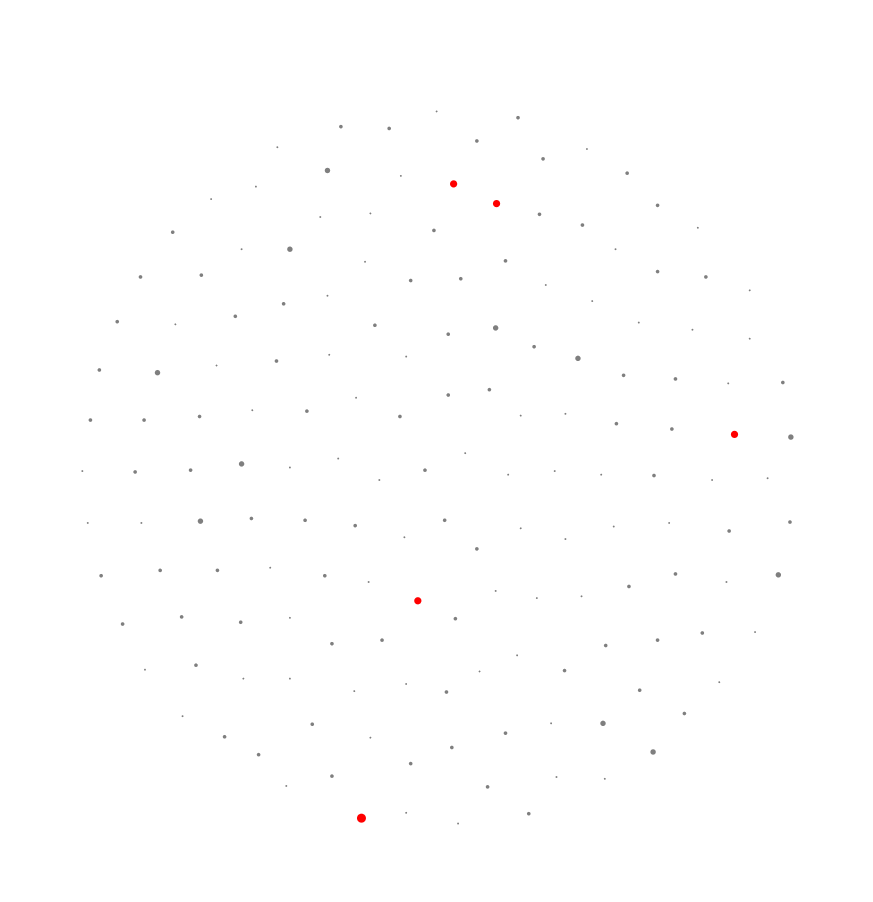
\includegraphics[scale=0.27]{figures/mondrian.png}
% \caption{The resulting GtMondrian visualization built with GT}
% \label{fig:mondrian}
% \end{figure}
% }
% \end{enumerate}
\ifthenelse{\boolean{showsolution}}{\newpage}{}

\subsection*{Exercise 3: Detection of eager tests (3 pts)}
Your task is to extract all JUnit 3 tests from \texttt{modelWeka} that suffer from the ``Eager Test'' code smell. That is, you have to find every method with \texttt{\#isJUnit3Test} set to \texttt{true} that contains an assertion statement at least two times.
\solution{\texttt{tests := modelWeka allModelMethods select: \#isJUnit3Test.\\
eagerTests := tests select: [ : m \textbar\\
\hspace*{0.5cm}\textbar~asserts astNode~\textbar\\
\hspace*{0.5cm}asserts := OrderedCollection new.\\
\hspace*{0.5cm}astNode := m gtASTNode.\\
\hspace*{0.5cm}astNode\\
\hspace*{1.0cm}ifNotNil: [ astNode\\
\hspace*{1.5cm}allNodesOfType: JavaMethodInvocationNode\\
\hspace*{1.5cm}do: [ :node \textbar \\
\hspace*{2.0cm}(node name value beginsWith: \textquotesingle assert\textquotesingle)\\
\hspace*{2.5cm}ifTrue: [ asserts add: node ] ] ].\\
\hspace*{0.5cm}asserts size \textgreater~1 ].}}

% \subsection*{Exercise 5: Detection of eager tests (StringTest) (3 pts BONUS)}
% Your task is to list all methods in GT's class \texttt{StringTest} that suffer from the ``eager test'' code smell. That is, you have to find every method that contains at least two times an assertion statement in its code.\\\\
% \emph{NB: \texttt{StringTest} is the test class for the class \texttt{String}.}
% \solution{\texttt{eagerTests := OrderedCollection new.\\
% StringTest methodDict keysAndValuesDo: [ :k :v \textbar\\
% \hspace*{0.5cm}firstLocation := v asString findString: \textquotesingle assert:\textquotesingle.\\
% \hspace*{0.5cm}lastLocation := v asString findLastOccurrenceOfString: \textquotesingle assert:\textquotesingle\\
% \hspace*{1.0cm}startingAt: 1.\\
% \hspace*{0.5cm}(firstLocation \texttildelow= 0 and: firstLocation \texttildelow= lastLocation)\\
% \hspace*{1.0cm}ifTrue: [eagerTests add: k]].\\
% eagerTests.}}

% Solution with AST traversal:
% StringTest methods select: [: m |
% 	| visitor |
% 	visitor := EagerTestCounter new.
% 	m parseTree acceptVisitor: visitor.
% 	visitor count > 1 ]
%
%'From Pharo8.0.0 of 9 August 2020 [Build information: Pharo-8.0.0+build.1141.sha.1b7a8d8203fce2a57794451f555bba4222614081 (64 Bit)] on 3 November 2020 at 3:01:28.661308 pm'!
% RBProgramNodeVisitor subclass: #EagerTestCounter
% 	instanceVariableNames: 'count'
% 	classVariableNames: ''
% 	package: 'SMA-ForGt-Moose'!
% !EagerTestCounter methodsFor: 'accessing' stamp: 'GlamorousAuthor 11/3/2020 14:57'!
% visitMessageNode: aMessageNode
% 	(aMessageNode selector beginsWith: 'assert')
% 		ifTrue: [ count := count + 1 ]! !
% !EagerTestCounter methodsFor: 'accessing' stamp: 'GlamorousAuthor 11/3/2020 14:58'!
% initialize
% 	super initialize.
% 	count := 0! !
% !EagerTestCounter methodsFor: 'accessing' stamp: 'GlamorousAuthor 11/3/2020 14:59'!
% count
% 	^ count! !

\end{document}
